\subsection{Channel stop and field oxide}

The channel-stop is material with the primary function to limit the spread of the channel area and to prevent the formation of parasitic channels.
It is a highly doped p+ area.
On top of the channel stop impurities is a thick layer of silicon oxide which has the primary function of isolating all the transistors from each other.

Its top view and cross section can be seen below.

\begin{center}
	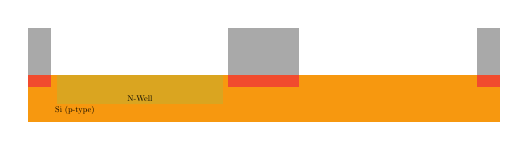
\begin{tikzpicture}[node distance = 3cm, auto, thick,scale=0.3, every node/.style={transform shape}]
		% substrate
		\fill[YellowOrange] (0,0) rectangle (20,2);
		\node at (2,0.5) {Si (p-type)};
		% n-well
		\fill[Goldenrod] (1.25,0.75) rectangle (8.25,2);
		\node at (4.75,1) {N-Well};
		% channel stop
		\fill[RedOrange] (0,1.5) rectangle (1,2);
		\fill[RedOrange] (8.5,1.5) rectangle (11.5,2);
		\fill[RedOrange] (19,1.5) rectangle (20,2);
		%field oxides:
		\fill[DarkGray] (0,2) rectangle (1,4);
		\fill[DarkGray] (8.5,2) rectangle (11.5,4);
		\fill[DarkGray] (19,2) rectangle (20,4);
	\end{tikzpicture}
	
\begin{tikzpicture}[node distance = 3cm, auto, thick,scale=0.3, every node/.style={transform shape}]
		% substrate
		\fill[YellowOrange] (0,0) rectangle (20,12);
		% n-well
		\fill[Goldenrod] (1.25,1.5) rectangle (8.25,7.25);
		% field oxide
		\fill[DarkGray] (0,0) rectangle (1,12);
		\fill[DarkGray] (8.5,0) rectangle (11.5,12);
		\fill[DarkGray] (19,0) rectangle (20,12);
		\fill[DarkGray] (0,0) rectangle (20,1.25);
		\fill[DarkGray] (0,7.5) rectangle (20,12);
	\end{tikzpicture}
\end{center}

It surrounds all the active areas and covers all the non-active area.
The channel-stop region is always accompanied by the field oxide layer and shares the same layout mask with it.

\subsubsection{Dioxide layer}
\begin{center}
	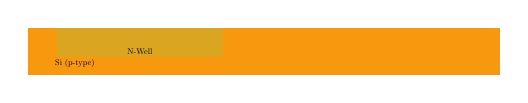
\begin{tikzpicture}[node distance = 3cm, auto, thick,scale=0.3, every node/.style={transform shape}]
		% substrate
		\fill[YellowOrange] (0,0) rectangle (20,2);
		\node at (2,0.5) {Si (p-type)};
		% n-well
		\fill[Goldenrod] (1.25,0.75) rectangle (8.25,2);
		\node at (4.75,1) {N-Well};
	\end{tikzpicture}

	\includegraphics[scale=0.01]{down_arrow.png}

	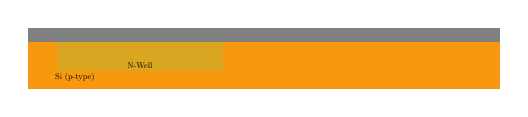
\begin{tikzpicture}[node distance = 3cm, auto, thick,scale=0.3, every node/.style={transform shape}]
		% substrate
		\fill[YellowOrange] (0,0) rectangle (20,2);
		\node at (2,0.5) {Si (p-type)};
		% n-well
		\fill[Goldenrod] (1.25,0.75) rectangle (8.25,2);
		\node at (4.75,1) {N-Well};
		% oxide
		\fill[gray] (0,2) rectangle (20,2.6);
	\end{tikzpicture}
\end{center}

\subsubsection{Nitride layer}
\begin{center}
	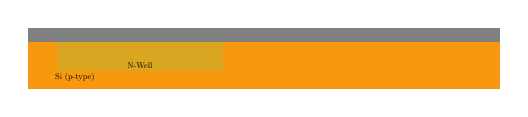
\begin{tikzpicture}[node distance = 3cm, auto, thick,scale=0.3, every node/.style={transform shape}]
		% substrate
		\fill[YellowOrange] (0,0) rectangle (20,2);
		\node at (2,0.5) {Si (p-type)};
		% n-well
		\fill[Goldenrod] (1.25,0.75) rectangle (8.25,2);
		\node at (4.75,1) {N-Well};
		% oxide
		\fill[gray] (0,2) rectangle (20,2.6);
	\end{tikzpicture}

	\includegraphics[scale=0.01]{down_arrow.png}

	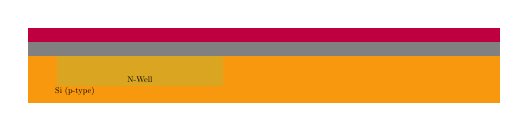
\begin{tikzpicture}[node distance = 3cm, auto, thick,scale=0.3, every node/.style={transform shape}]
		% substrate
		\fill[YellowOrange] (0,0) rectangle (20,2);
		\node at (2,0.5) {Si (p-type)};
		% n-well
		\fill[Goldenrod] (1.25,0.75) rectangle (8.25,2);
		\node at (4.75,1) {N-Well};
		% oxide
		\fill[gray] (0,2) rectangle (20,2.6);
		% nitride
		\fill[purple] (0,2.6) rectangle (20,3.2);
	\end{tikzpicture}
\end{center}

\subsubsection{Patterning}
\begin{center}
	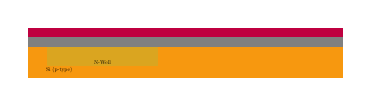
\begin{tikzpicture}[node distance = 3cm, auto, thick,scale=0.2, every node/.style={transform shape}]
		% substrate
		\fill[YellowOrange] (0,0) rectangle (20,2);
		\node at (2,0.5) {Si (p-type)};
		% n-well
		\fill[Goldenrod] (1.25,0.75) rectangle (8.25,2);
		\node at (4.75,1) {N-Well};
		% oxide
		\fill[gray] (0,2) rectangle (20,2.6);
		% nitride
		\fill[purple] (0,2.6) rectangle (20,3.2);
	\end{tikzpicture}
	
\begin{tikzpicture}[node distance = 3cm, auto, thick,scale=0.2, every node/.style={transform shape}]
		\fill[purple] (0,0) rectangle (20,12);
	\end{tikzpicture}

	\includegraphics[scale=0.01]{down_arrow.png}

	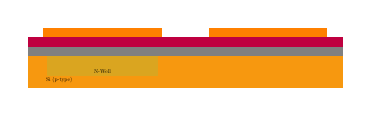
\begin{tikzpicture}[node distance = 3cm, auto, thick,scale=0.2, every node/.style={transform shape}]
		% substrate
		\fill[YellowOrange] (0,0) rectangle (20,2);
		\node at (2,0.5) {Si (p-type)};
		% n-well
		\fill[Goldenrod] (1.25,0.75) rectangle (8.25,2);
		\node at (4.75,1) {N-Well};
		% oxide
		\fill[gray] (0,2) rectangle (20,2.6);
		% nitride
		\fill[purple] (0,2.6) rectangle (20,3.2);
		% resist
		\fill[orange] (1,3.2) rectangle (8.5,3.8);
		\fill[orange] (11.5,3.2) rectangle (19,3.8);
	\end{tikzpicture}
	
\begin{tikzpicture}[node distance = 3cm, auto, thick,scale=0.2, every node/.style={transform shape}]
		\fill[purple] (0,0) rectangle (20,12);
		\fill[orange] (1,1.25) rectangle (8.5,7.5);
		\fill[orange] (11.5,1.25) rectangle (19,7.5);
	\end{tikzpicture}
\end{center}

\subsubsection{Etching}
\begin{center}
	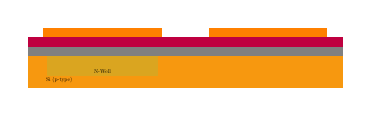
\begin{tikzpicture}[node distance = 3cm, auto, thick,scale=0.2, every node/.style={transform shape}]
		% substrate
		\fill[YellowOrange] (0,0) rectangle (20,2);
		\node at (2,0.5) {Si (p-type)};
		% n-well
		\fill[Goldenrod] (1.25,0.75) rectangle (8.25,2);
		\node at (4.75,1) {N-Well};
		% oxide
		\fill[gray] (0,2) rectangle (20,2.6);
		% nitride
		\fill[purple] (0,2.6) rectangle (20,3.2);
		% resist
		\fill[orange] (1,3.2) rectangle (8.5,3.8);
		\fill[orange] (11.5,3.2) rectangle (19,3.8);
	\end{tikzpicture}
	
\begin{tikzpicture}[node distance = 3cm, auto, thick,scale=0.2, every node/.style={transform shape}]
		\fill[purple] (0,0) rectangle (20,12);
		\fill[orange] (1,1.25) rectangle (8.5,7.5);
		\fill[orange] (11.5,1.25) rectangle (19,7.5);
	\end{tikzpicture}

	\includegraphics[scale=0.01]{down_arrow.png}

	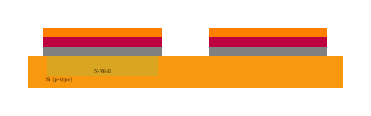
\begin{tikzpicture}[node distance = 3cm, auto, thick,scale=0.2, every node/.style={transform shape}]
		% substrate
		\fill[YellowOrange] (0,0) rectangle (20,2);
		\node at (2,0.5) {Si (p-type)};
		% n-well
		\fill[Goldenrod] (1.25,0.75) rectangle (8.25,2);
		\node at (4.75,1) {N-Well};
		% oxide
		\fill[gray] (1,2) rectangle (8.5,2.6);
		\fill[gray] (11.5,2) rectangle (19,2.6);
		% nitride
		\fill[purple] (1,2.6) rectangle (8.5,3.2);
		\fill[purple] (11.5,2.6) rectangle (19,3.2);
		% resist
		\fill[orange] (1,3.2) rectangle (8.5,3.8);
		\fill[orange] (11.5,3.2) rectangle (19,3.8);
	\end{tikzpicture}
	
\begin{tikzpicture}[node distance = 3cm, auto, thick,scale=0.2, every node/.style={transform shape}]
		\fill[YellowOrange] (0,0) rectangle (20,12);
		\fill[orange] (1,1.25) rectangle (8.5,7.5);
		\fill[orange] (11.5,1.25) rectangle (19,7.5);
	\end{tikzpicture}
\end{center}

\subsubsection{Cleaning}
\begin{center}
	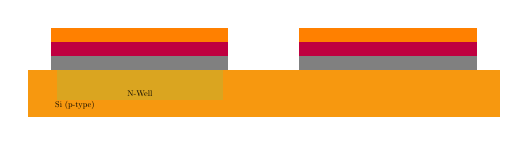
\begin{tikzpicture}[node distance = 3cm, auto, thick,scale=0.3, every node/.style={transform shape}]
		% substrate
		\fill[YellowOrange] (0,0) rectangle (20,2);
		\node at (2,0.5) {Si (p-type)};
		% n-well
		\fill[Goldenrod] (1.25,0.75) rectangle (8.25,2);
		\node at (4.75,1) {N-Well};
		% oxide
		\fill[gray] (1,2) rectangle (8.5,2.6);
		\fill[gray] (11.5,2) rectangle (19,2.6);
		% nitride
		\fill[purple] (1,2.6) rectangle (8.5,3.2);
		\fill[purple] (11.5,2.6) rectangle (19,3.2);
		% resist
		\fill[orange] (1,3.2) rectangle (8.5,3.8);
		\fill[orange] (11.5,3.2) rectangle (19,3.8);
	\end{tikzpicture}

	\includegraphics[scale=0.01]{down_arrow.png}

	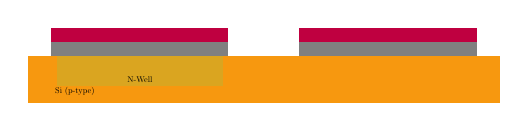
\begin{tikzpicture}[node distance = 3cm, auto, thick,scale=0.3, every node/.style={transform shape}]
		% substrate
		\fill[YellowOrange] (0,0) rectangle (20,2);
		\node at (2,0.5) {Si (p-type)};
		% n-well
		\fill[Goldenrod] (1.25,0.75) rectangle (8.25,2);
		\node at (4.75,1) {N-Well};
		% oxide
		\fill[gray] (1,2) rectangle (8.5,2.6);
		\fill[gray] (11.5,2) rectangle (19,2.6);
		% nitride
		\fill[purple] (1,2.6) rectangle (8.5,3.2);
		\fill[purple] (11.5,2.6) rectangle (19,3.2);
	\end{tikzpicture}
\end{center}

\subsubsection{Predeposition}
\begin{center}
	\begin{tikzpicture}[node distance = 3cm, auto, thick,scale=0.3, every node/.style={transform shape}]
		% substrate
		\fill[YellowOrange] (0,0) rectangle (20,2);
		\node at (2,0.5) {Si (p-type)};
		% n-well
		\fill[Goldenrod] (1.25,0.75) rectangle (8.25,2);
		\node at (4.75,1) {N-Well};
		% oxide
		\fill[gray] (1,2) rectangle (8.5,2.6);
		\fill[gray] (11.5,2) rectangle (19,2.6);
		% nitride
		\fill[purple] (1,2.6) rectangle (8.5,3.2);
		\fill[purple] (11.5,2.6) rectangle (19,3.2);

		\forloop{ct}{0}{\value{ct} < 21}
		{
			\draw [->] (\value{ct},4.5) -- (\value{ct},3.5);
			\node at (\value{ct},4.8) {B$^{11}$};
		}
	\end{tikzpicture}

	\includegraphics[scale=0.01]{down_arrow.png}

	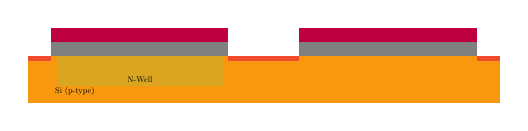
\begin{tikzpicture}[node distance = 3cm, auto, thick,scale=0.3, every node/.style={transform shape}]
		% substrate
		\fill[YellowOrange] (0,0) rectangle (20,2);
		\node at (2,0.5) {Si (p-type)};
		% n-well
		\fill[Goldenrod] (1.25,0.75) rectangle (8.25,2);
		\node at (4.75,1) {N-Well};
		% oxide
		\fill[gray] (1,2) rectangle (8.5,2.6);
		\fill[gray] (11.5,2) rectangle (19,2.6);
		% nitride
		\fill[purple] (1,2.6) rectangle (8.5,3.2);
		\fill[purple] (11.5,2.6) rectangle (19,3.2);
		% channel stop
		\fill[RedOrange] (0,1.8) rectangle (1,2);
		\fill[RedOrange] (8.5,1.8) rectangle (11.5,2);
		\fill[RedOrange] (19,1.8) rectangle (20,2);
	\end{tikzpicture}
\end{center}

\subsubsection{Thick oxide layer}
\begin{center}
	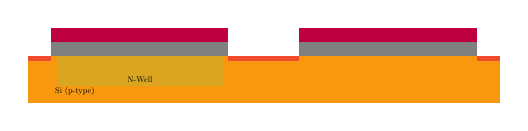
\begin{tikzpicture}[node distance = 3cm, auto, thick,scale=0.3, every node/.style={transform shape}]
		% substrate
		\fill[YellowOrange] (0,0) rectangle (20,2);
		\node at (2,0.5) {Si (p-type)};
		% n-well
		\fill[Goldenrod] (1.25,0.75) rectangle (8.25,2);
		\node at (4.75,1) {N-Well};
		% oxide
		\fill[gray] (1,2) rectangle (8.5,2.6);
		\fill[gray] (11.5,2) rectangle (19,2.6);
		% nitride
		\fill[purple] (1,2.6) rectangle (8.5,3.2);
		\fill[purple] (11.5,2.6) rectangle (19,3.2);
		% channel stop
		\fill[RedOrange] (0,1.8) rectangle (1,2);
		\fill[RedOrange] (8.5,1.8) rectangle (11.5,2);
		\fill[RedOrange] (19,1.8) rectangle (20,2);
	\end{tikzpicture}

	\includegraphics[scale=0.01]{down_arrow.png}

	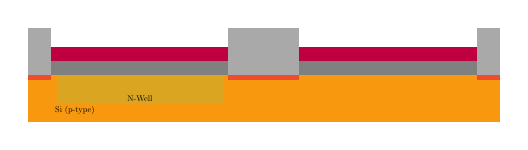
\begin{tikzpicture}[node distance = 3cm, auto, thick,scale=0.3, every node/.style={transform shape}]
		% substrate
		\fill[YellowOrange] (0,0) rectangle (20,2);
		\node at (2,0.5) {Si (p-type)};
		% n-well
		\fill[Goldenrod] (1.25,0.75) rectangle (8.25,2);
		\node at (4.75,1) {N-Well};
		% oxide
		\fill[gray] (1,2) rectangle (8.5,2.6);
		\fill[gray] (11.5,2) rectangle (19,2.6);
		% nitride
		\fill[purple] (1,2.6) rectangle (8.5,3.2);
		\fill[purple] (11.5,2.6) rectangle (19,3.2);
		% channel stop
		\fill[RedOrange] (0,1.8) rectangle (1,2);
		\fill[RedOrange] (8.5,1.8) rectangle (11.5,2);
		\fill[RedOrange] (19,1.8) rectangle (20,2);
		%field oxides:
		\fill[DarkGray] (0,2) rectangle (1,4);
		\fill[DarkGray] (8.5,2) rectangle (11.5,4);
		\fill[DarkGray] (19,2) rectangle (20,4);
	\end{tikzpicture}
\end{center}

\subsubsection{Infusion}
\begin{center}
	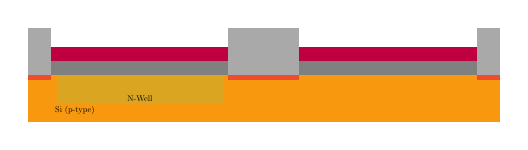
\begin{tikzpicture}[node distance = 3cm, auto, thick,scale=0.3, every node/.style={transform shape}]
		% substrate
		\fill[YellowOrange] (0,0) rectangle (20,2);
		\node at (2,0.5) {Si (p-type)};
		% n-well
		\fill[Goldenrod] (1.25,0.75) rectangle (8.25,2);
		\node at (4.75,1) {N-Well};
		% oxide
		\fill[gray] (1,2) rectangle (8.5,2.6);
		\fill[gray] (11.5,2) rectangle (19,2.6);
		% nitride
		\fill[purple] (1,2.6) rectangle (8.5,3.2);
		\fill[purple] (11.5,2.6) rectangle (19,3.2);
		% channel stop
		\fill[RedOrange] (0,1.8) rectangle (1,2);
		\fill[RedOrange] (8.5,1.8) rectangle (11.5,2);
		\fill[RedOrange] (19,1.8) rectangle (20,2);
		%field oxides:
		\fill[DarkGray] (0,2) rectangle (1,4);
		\fill[DarkGray] (8.5,2) rectangle (11.5,4);
		\fill[DarkGray] (19,2) rectangle (20,4);
	\end{tikzpicture}

	\includegraphics[scale=0.01]{down_arrow.png}

	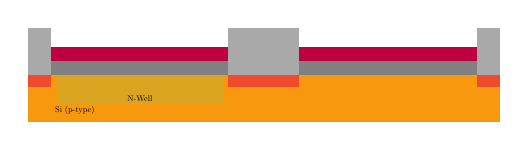
\begin{tikzpicture}[node distance = 3cm, auto, thick,scale=0.3, every node/.style={transform shape}]
		% substrate
		\fill[YellowOrange] (0,0) rectangle (20,2);
		\node at (2,0.5) {Si (p-type)};
		% n-well
		\fill[Goldenrod] (1.25,0.75) rectangle (8.25,2);
		\node at (4.75,1) {N-Well};
		% oxide
		\fill[gray] (1,2) rectangle (8.5,2.6);
		\fill[gray] (11.5,2) rectangle (19,2.6);
		% nitride
		\fill[purple] (1,2.6) rectangle (8.5,3.2);
		\fill[purple] (11.5,2.6) rectangle (19,3.2);
		% channel stop
		\fill[RedOrange] (0,1.5) rectangle (1,2);
		\fill[RedOrange] (8.5,1.5) rectangle (11.5,2);
		\fill[RedOrange] (19,1.5) rectangle (20,2);
		%field oxides:
		\fill[DarkGray] (0,2) rectangle (1,4);
		\fill[DarkGray] (8.5,2) rectangle (11.5,4);
		\fill[DarkGray] (19,2) rectangle (20,4);
	\end{tikzpicture}
\end{center}

\subsubsection{Patterning}
\begin{center}
	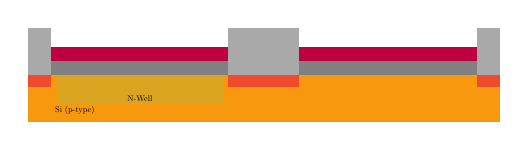
\begin{tikzpicture}[node distance = 3cm, auto, thick,scale=0.3, every node/.style={transform shape}]
		% substrate
		\fill[YellowOrange] (0,0) rectangle (20,2);
		\node at (2,0.5) {Si (p-type)};
		% n-well
		\fill[Goldenrod] (1.25,0.75) rectangle (8.25,2);
		\node at (4.75,1) {N-Well};
		% oxide
		\fill[gray] (1,2) rectangle (8.5,2.6);
		\fill[gray] (11.5,2) rectangle (19,2.6);
		% nitride
		\fill[purple] (1,2.6) rectangle (8.5,3.2);
		\fill[purple] (11.5,2.6) rectangle (19,3.2);
		% channel stop
		\fill[RedOrange] (0,1.5) rectangle (1,2);
		\fill[RedOrange] (8.5,1.5) rectangle (11.5,2);
		\fill[RedOrange] (19,1.5) rectangle (20,2);
		%field oxides:
		\fill[DarkGray] (0,2) rectangle (1,4);
		\fill[DarkGray] (8.5,2) rectangle (11.5,4);
		\fill[DarkGray] (19,2) rectangle (20,4);
	\end{tikzpicture}

	\includegraphics[scale=0.01]{down_arrow.png}

	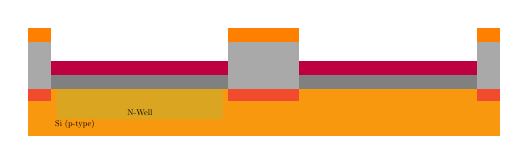
\begin{tikzpicture}[node distance = 3cm, auto, thick,scale=0.3, every node/.style={transform shape}]
		% substrate
		\fill[YellowOrange] (0,0) rectangle (20,2);
		\node at (2,0.5) {Si (p-type)};
		% n-well
		\fill[Goldenrod] (1.25,0.75) rectangle (8.25,2);
		\node at (4.75,1) {N-Well};
		% oxide
		\fill[gray] (1,2) rectangle (8.5,2.6);
		\fill[gray] (11.5,2) rectangle (19,2.6);
		% nitride
		\fill[purple] (1,2.6) rectangle (8.5,3.2);
		\fill[purple] (11.5,2.6) rectangle (19,3.2);
		% channel stop
		\fill[RedOrange] (0,1.5) rectangle (1,2);
		\fill[RedOrange] (8.5,1.5) rectangle (11.5,2);
		\fill[RedOrange] (19,1.5) rectangle (20,2);
		%field oxides:
		\fill[DarkGray] (0,2) rectangle (1,4);
		\fill[DarkGray] (8.5,2) rectangle (11.5,4);
		\fill[DarkGray] (19,2) rectangle (20,4);
		% resist
		\fill[orange] (0,4) rectangle (1,4.6);
		\fill[orange] (8.5,4) rectangle (11.5,4.6);
		\fill[orange] (19,4) rectangle (20,4.6);
	\end{tikzpicture}
\end{center}

\subsubsection{Etching}
\begin{center}
	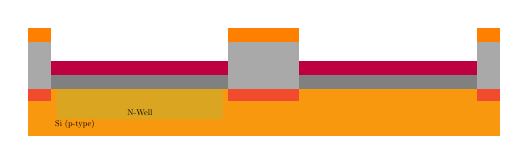
\begin{tikzpicture}[node distance = 3cm, auto, thick,scale=0.3, every node/.style={transform shape}]
		% substrate
		\fill[YellowOrange] (0,0) rectangle (20,2);
		\node at (2,0.5) {Si (p-type)};
		% n-well
		\fill[Goldenrod] (1.25,0.75) rectangle (8.25,2);
		\node at (4.75,1) {N-Well};
		% oxide
		\fill[gray] (1,2) rectangle (8.5,2.6);
		\fill[gray] (11.5,2) rectangle (19,2.6);
		% nitride
		\fill[purple] (1,2.6) rectangle (8.5,3.2);
		\fill[purple] (11.5,2.6) rectangle (19,3.2);
		% channel stop
		\fill[RedOrange] (0,1.5) rectangle (1,2);
		\fill[RedOrange] (8.5,1.5) rectangle (11.5,2);
		\fill[RedOrange] (19,1.5) rectangle (20,2);
		%field oxides:
		\fill[DarkGray] (0,2) rectangle (1,4);
		\fill[DarkGray] (8.5,2) rectangle (11.5,4);
		\fill[DarkGray] (19,2) rectangle (20,4);
		% resist
		\fill[orange] (0,4) rectangle (1,4.6);
		\fill[orange] (8.5,4) rectangle (11.5,4.6);
		\fill[orange] (19,4) rectangle (20,4.6);
	\end{tikzpicture}

	\includegraphics[scale=0.01]{down_arrow.png}

	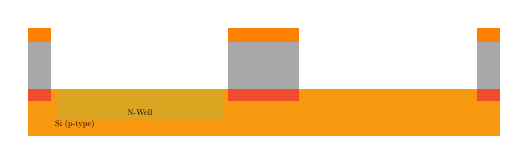
\begin{tikzpicture}[node distance = 3cm, auto, thick,scale=0.3, every node/.style={transform shape}]
		% substrate
		\fill[YellowOrange] (0,0) rectangle (20,2);
		\node at (2,0.5) {Si (p-type)};
		% n-well
		\fill[Goldenrod] (1.25,0.75) rectangle (8.25,2);
		\node at (4.75,1) {N-Well};
		% channel stop
		\fill[RedOrange] (0,1.5) rectangle (1,2);
		\fill[RedOrange] (8.5,1.5) rectangle (11.5,2);
		\fill[RedOrange] (19,1.5) rectangle (20,2);
		%field oxides:
		\fill[DarkGray] (0,2) rectangle (1,4);
		\fill[DarkGray] (8.5,2) rectangle (11.5,4);
		\fill[DarkGray] (19,2) rectangle (20,4);
		% resist
		\fill[orange] (0,4) rectangle (1,4.6);
		\fill[orange] (8.5,4) rectangle (11.5,4.6);
		\fill[orange] (19,4) rectangle (20,4.6);
	\end{tikzpicture}
\end{center}